
Many figures in this document? were produced using MATLAB, for example: fig +++++++. In this appendix, we will give a brief tutorial on their production. Fast-slow systems like the ones studied here are a classic example of \emph{stiff} ODEs\footnote{Indeed, the MATLAB documentation for its stiff solver, \texttt{ode15s}, uses the Van Der Pol equation as it's example.}. 
\begin{definition}[Stiffness Ratio]
	Consider $\dot{x} = F(x)$ where $x\in \mathbf{R}^n, F\in C^r(\mathbf{R}^n,\mathbf{R}^n)$. Let 
	$$ x' = Ax,\quad A\in \mathbf{R}^{n \times n}  $$
	denote its linearisation. Suppose all the eigenvalues $\lambda_j$  of $A$ have negative real parts. Then the \emph{stiffness ratio}, $\mu$ is defined as
	$$ \mu :=\frac{\max_j(\mathrm{Re}(\lambda_j))}{\min_j(\mathrm{Re}(\lambda_j))} $$
	If $\mu$ is large, the system is called \emph{stiff}.
\end{definition}
Stiffness is not a well-defined concept, it can be seen as a general term for a set of equations which are difficult to solve numerically to a high level of accuracy. Throughout this section we will consider the general problem above as an initial value problem.

$$ \begin{cases}
\dot{x} = F(x)\\
x(T_0)=x_0
\end{cases}$$
As before, $x\in \mathbf{R}^n$ and $ F\in C^r(\mathbf{R}^n,\mathbf{R}^n)$. To solve such a system numerically, time must be discretised. Using standard notation, let $h$ be the time step between points on the solution. To differentiate between the continuous solution $x(t)$ and the discretised solution, we denote the latter by $x(t_j)=x_j$. Here $t_j = T_0+jh$. As a first example, consider the modified Euler method.

$$ x(t_{n+1})=x(t_n)+hF\left( x(t_n) +\frac{1}{2}F(x(t_n))\right)$$
Or, in the more compact notation, 
$$x_{n+1}=x_n+hF\left( x_n +\frac{1}{2}F(x_n)\right)$$
This is a simple method and provides a starting point in considering error between true and numerical solutions.\\

The go-to ODE solver in MATLAB is \texttt{ode45}. This function uses the Dormand-Prince Runge-Kutta method, an explicit single-step formula. The Runge-Kutta method (RK4) is similar to the explicit Euler method in that it calculates the next point ($x_{n+1}$) using only its current value ($x_n$). Unlike the Euler method however, it yields much lower error by using a better approximation of the derivative at points in between $x_n$ and $x_{n+1}$ as opposed to only the derivative at the initial point. The Runge-Kutta method uses the following relation.


$$ x_{n+1} = x_n +\frac{1}{6} h \left(k_1+2k_2+2k_3+k_4\right)$$
where
\begin{align*}
k_1 &= F(x_n)\\
k_2 &= F\left(x_n+\frac{1}{2}hk_1\right)\\
k_3 &= F\left(x_n +\frac{1}{2}hk_2\right)\\
k_4 &= F\left(x_n + hk_3\right)
\end{align*}
The Runge-Kutta family of solvers are ubiquitous in numerical analysis, and most methods can be categorised as belonging to this set of methods. Even the simplest, the explicit Euler scheme, is a RK method. Note that \texttt{ode45} doesn't use RK4, it uses an adaptive method that repeats steps if the error in the step is too high. This produces an even more accurate solution without adding much computational cost. \\

Let's look at the use of these various methods on the simplest fast-slow system.
		\begin{equation} \begin{cases}
		\begin{pmatrix} \dot{x}\\\dot{y}\end{pmatrix}=\begin{pmatrix}
		-1/\epsilon & 0 \\
		0& -1
		\end{pmatrix}\begin{pmatrix}
		x\\y 
		\end{pmatrix}\\
		(x(0),y(0))= (x_0,y_0)
		\end{cases}\label{eq:test}\end{equation}
This system has an easy analytic solution, $x(t) = x_0\exp(-t/\epsilon), y(t)=y_0 \exp(-t)$. For this reason it is a useful test system with which to analyse the convergence of numerical schemes. The stiffness ratio for this system is
$$ \mu =\frac{\max_j(\mathrm{Re}(\lambda_j))}{\min_j(\mathrm{Re}(\lambda_j))}= \frac{1}{\epsilon} $$
The time separation, $\epsilon \ll 1$ and so this system is very stiff. We thus expect explicit solvers to perform poorly. +++Explain about convergence here? Would be nice to do for modEuler and RK4 too+++.\\
The lack of stability of these algorithms in practice, even for very simple systems, clearly necessitates the introduction of alternative methods.
\begin{figure}
	\centering
	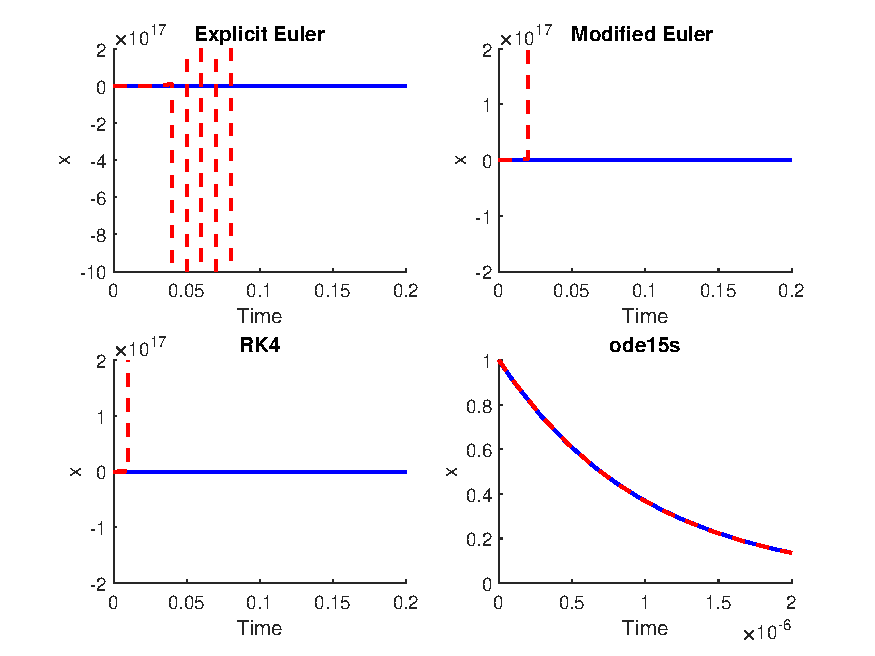
\includegraphics[width=0.8\linewidth]{TestEqSim}
	\caption[Numerical Stability Comparison]{Comparison of stability of different numerical schemes applied to Equation \ref{eq:test}. Blue solid line indicates analytic solution, dashed red indicates numeric solution using the scheme given in the plot title. Note the varying scales on the axes.}
	
\end{figure}

\subsection{Stiff Solvers}
\begin{figure}
	\centering
	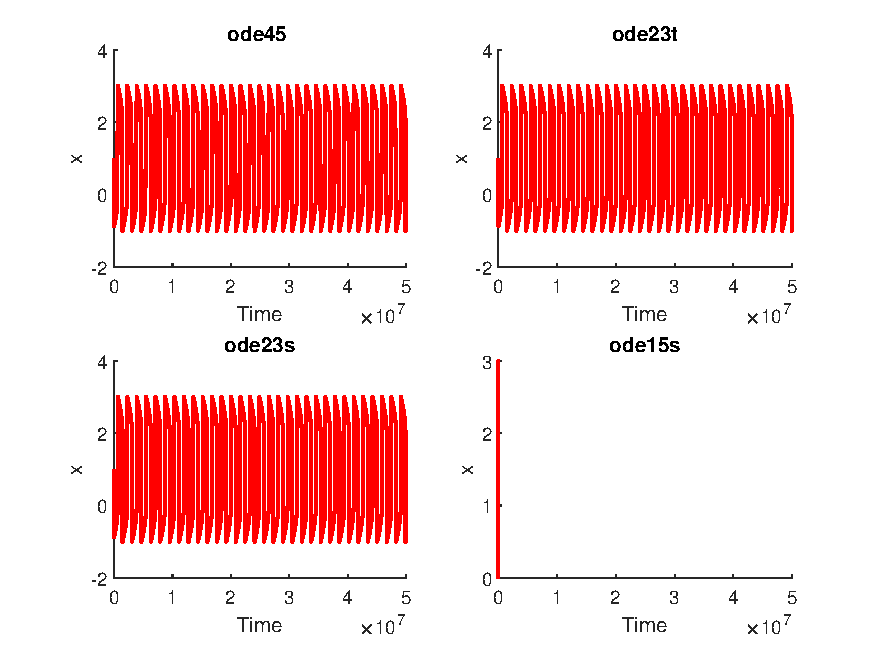
\includegraphics[width=0.8\linewidth]{stiffVDP.pdf}
	\caption[Stiff Solvers]{Comparison of stiff solvers for VDP. +++Note all get correct trajectory, what about speed?+++.}
	
\end{figure}

+++\texttt{ode15s,ode23t,ode23s} use, comparison of speed with \texttt{ode45}. Note difference between RK4.+++



		Test on RK4, mod-Euler and \texttt{ode15s}? Intro BDF? Check sec8 MMO.

